\textbf{Another alternative approximation problem:} Find a linear function $l(x)$ such that \[\max_{0\le x\le 1} |\mathrm{e}^x - l(x)| = \min.\]

{\color{blue}

We find the values for $f(x) = \mathrm{e}^x - a\, x - b$ where the
difference is large.

\[
\begin{aligned}
f(x) &= |\mathrm{e}^x - a\, x - b| \\
f(0) &= | 1 - b | \\
f(1) &= | \mathrm{e} - a - b| \\
f(\log a) &= | \mathrm{e}^{\log a} - a\, \log a - b| \\
&= | a - a\, \log a - b |
\end{aligned}
\]

By setting these equations equal to each other, we can eliminate
variables, and find the values for $a$ and $b$ that minimize $f(x)$.

\[
\begin{aligned}
1 - b &= \mathrm{e} - a - b \\
\Rightarrow a &= \mathrm{e} - 1
\end{aligned}
\]

\[
\begin{aligned}
b - 1 &= a - a \log a - b \\
2b &= 1 + a - a \log a \\
&= 1 + (\mathrm{e} - 1) - (\mathrm{e} -1) \log (\mathrm{e} - 1) \\
&= \mathrm{e} - (\mathrm{e} -1) \log (\mathrm{e} - 1) \\
\Rightarrow b &=
\frac{\mathrm{e} - (\mathrm{e} -1) \log (\mathrm{e} - 1)}{2} \\
\end{aligned}
\]

\[
l(x) =
\left(\mathrm{e} - 1\right)\, x +
\frac{\mathrm{e} - (\mathrm{e} -1) \log (\mathrm{e} - 1)}{2} \\
\]

\begin{figure}[H]
\centering
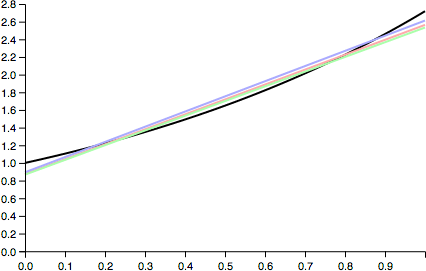
\includegraphics[scale=0.65]{approximations-of-e-x.png}
\caption{We plot $e^x$ in black, with the solutions to exercises 11 (red),
12 (green), and 13 (blue). We can visually see that our solutions all
linearly approximate $e^x$ on $[0,1]$.}
\end{figure}

}
